
\newthought{This} section discusses the motivation for exact determinations of eddy \textit{scales}. That is, their horizontal extent \ie their diameter or \textit{wavelength}.

 %%%%%%%%%%%%%%%%%%%%%%%%%%%%%%%%%%%%%%%%%%%%%%%%%%%%%%%%%%%%%%%%%%%%%%%%%%%%%%%%%
\begin{marginfigure}
	\label{fig:allEddies-aviIaviIIpop7II}
	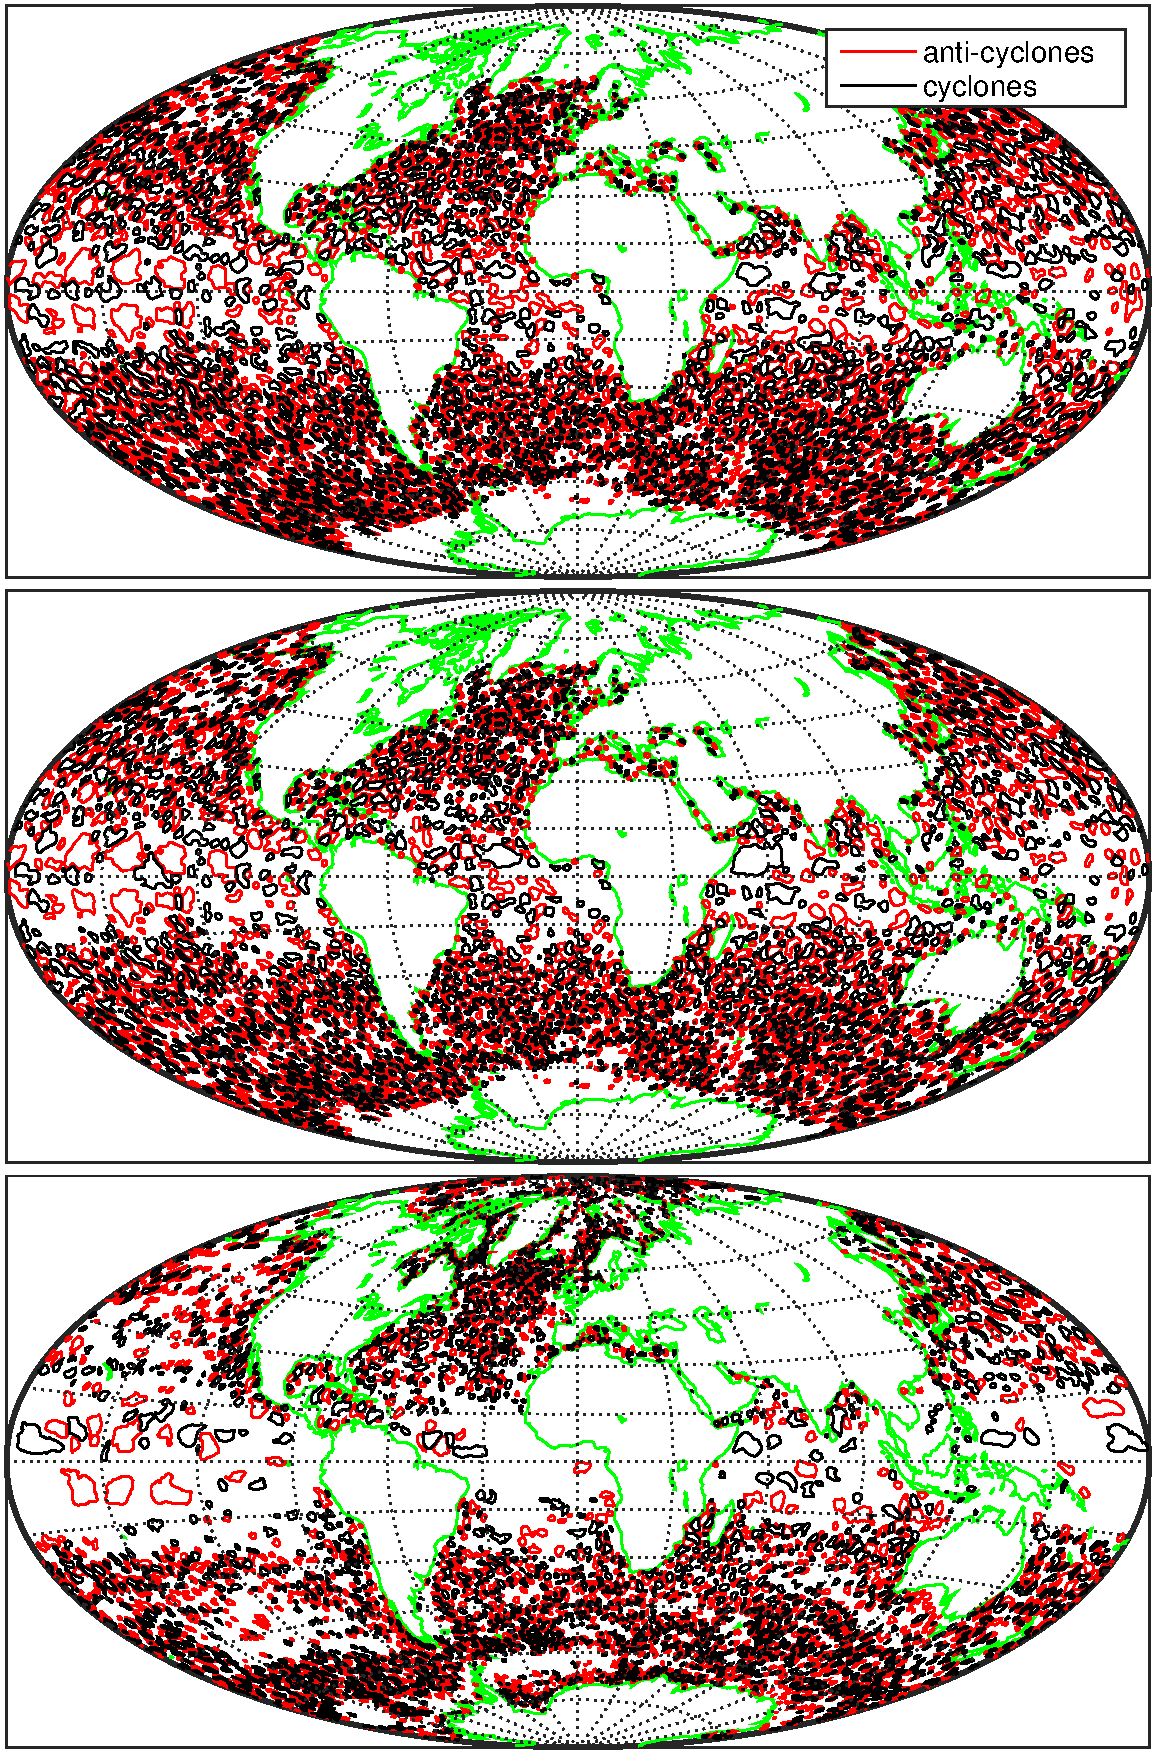
\includegraphics[]{allEddies-aviIaviIIpop7II}
	\caption{All contours that passed the filtering procedure for one exemplary time-step. Top: \aviI. Mid: \aviII. Bottom: \popSevenII.}
\end{marginfigure}
 %%%%%%%%%%%%%%%%%%%%%%%%%%%%%%%%%%%%%%%%%%%%%%%%%%%%%%%%%%%%%%%%%%%%%%%%%%%%%%%%%

%%%####################################################################
%%%####################################################################
\newthought{Just} like the eddy itself, its scale is rather vague and difficult to define. What physical parameter defines the outer edge of a seamless, smooth vortex? If the eddy is detected as done by \citet{Chelton2011}, \ie closed contours of \SSH, the interior of which fulfilling certain criteria, the measured perimeter may jump considerably from one time step to the next. An incremental difference in the choice of $z$ might translate to a perimeter outlining twice the  difference in area, especially when \SSH~gradients are small.\\
Another possibility is to define an amplitude first, then assume a certain shape \eg Gaussian, and then infer the radius indirectly. The obvious problem with this approach would be to properly define the amplitude.\\
The most physically sound method would have to be one depending on the eddy's most defining physical variable that is unambiguously determinable from \SSH: the geostrophic velocities. \citet{Chelton2011}, as with everything else, tried all methods but conclude that the later is the most adequate one \footnote{See \cref{filter:chstuff}}.

%%
%%%####################################################################
%%%####################################################################
%



\newthought{Construed} as an integral length scale of turbulence \ie as the distance at which the auto-correlation of particles reaches zero \citep{batchelor1969computation,Eden2007}, the eddy-\emph{scale} turns out to be of fundamental relevance for attempts to parameterize geostrophic turbulence.

\newthought{General circulation models}~($\order{2}\si{km}$) as they are used in \eg climate forecasts are too coarse to resolve mesoscale ($\order{1}\si{km}$) turbulence \citep{Eden2007a,Eden2007,Eden2006b,Treguier1997,Ferrari2010} . Even if the Von-Neumann-condition was ignored and a refinement was desired horizontally only, a leap of one order of magnitude would effect an increase in calculation time \footnote{With the Moore's-Law-type exponential growth in FLOP/S of the last 22 years for supercomputers ($\lg(x)\sim 3/11 a$) a factor $100$ interestingly translates to only $a=22/3\approx 7$ years...} of factor $x=100$.  The effects of the nonlinear terms therefore have to be somehow articulated in an integral sense for the large grid-boxes in the model \citep{Fox-Kemper2008,Marshall1981,gent1995parameterizing,Modeling,Gaspar1990,StephenM.Griffies2003,Sciences1999}.
A common approach is to assume that eddy kinetic energy $\ol{ \vec{u}'\vec{u}'}$ and eddy potential energy $\ol{  w'\rho'}$, akin to diffusive processes\footnote{In analogy to Fick's first law of diffusion.}
, were proportional to the gradient of $\ol{u}$ respective $\ol{b}$
(down-gradient-parameterization \footnote{\ie Reynolds averaging})
\citep{olbers2012ocean,Marshall2010,eden2012implementing}, which leads to the problem of finding expressions for the
\textit{turbulent diffusivities} \ie the rate at which gradients are diffused by turbulence. This parameter is by no means constant, instead it can span
several orders of magnitude, itself depending on the strength of turbulence-relevant gradients, and sometimes even assuming negative values
\citep{eden2008towards}. Precise knowledge of the integral length scale and the physics that set it is hence vital for attempts to analyze and set values for
eddy diffusivities and turbulence parameterizations in general.



%\TODO{[...] i took out section on eddy diffusivities}


%\newthought{Eddy Diffusivities} For simplicity assume full incompressibility and a variable density $\rho(T)$, that is linearly dependent on temperature only and that there be some radiative surface flux $J^{rad}$ for $T$, hence also for $\rho$. Further consider kinetic energy being burned to heat on molecular scales \ie Joule heating, creating another positive source of $T$ thus $\rho$. \derref{der:FIELDSDER}

%%%....................................................................
%\begin{subequations} \label{eq:inhomo_fin}
%\begin{align}
	%\dpr{\ol{\vec{u}_h}}{t}
	%+
	%\ol{ \dpr{w'\vec{u}_h'}{z}}
	%+
	%f \vec{k} \times \ol{\vec{u}_h}
	%&=
	%0 \\
		 %%%--------------------------------------------------------------------
	 %\dpr{\ol{\rho}}{t}
	 %&=
	 %-\dpr{}{z}
	 %\left(
%\ol{  w'\rho'}
%-\ol{\vec{J}}_{rad}
%+   \kappa \dpr{ \ol{\rho}}{z} \right)
%\end{align}
%\end{subequations}
%%%....................................................................
%\TODO{introduce buoyancy instead rho- for eq. of state}
%If the aim was to solve \eqsref{eq:inhomo_fin} numerically for the mean quantities, parametrizations for the \textit{eddy kinetic energy}-term $\ol{ w'\vec{u}_h'}$ and the \textit{eddy potential energy}-term \footnote{$\ol{  w'\rho'}$ is an exchange term between potential and kinetic energy} $\ol{  w'\rho'}$ would have to be found. A common approach is to assume that the turbulent energy, akin to diffusive processes\footnote{In analogy to Fick's first law of diffusion}, is proportional to the gradient of $\ol{u}$ respective $\ol{b}$  (down-gradient-parametrization) \citep*{olbers2012ocean}.
%%%....................................................................
%\begin{subequations} \label{eq:downgrad}
%\begin{align}
%\ol{ w'\vec{u}_h'}
%&=
%-K_u \dpr{\ol{\vec{u}}}{z} \\
  %%%--------------------------------------------------------------------
 %\ol{  w'b}
 %&=
  %-K_{b} \dpr{\ol{b}}{z}
%\end{align}
%\end{subequations}
%%%....................................................................
%which leads to the problem of finding expressions for the turbulent diffusivities $K$. Heuristic considerations \citep{olbers2012ocean} suggest that $K \sim UL \sim \sqrt{E_t} L$ with the turbulent kinetic energy $E_t \sim \ol{u'u'}$. Assuming for now that the characteristic length scale $L$ is known and that the proportionality factors $c$ could be determined empirically, we still need to find an expression for $\Ek$. With $\star$ for either $u$ or $b$:
%%%....................................................................

%\begin{align}
%K_{\star}
%&=
%c_{\star} \sqrt{E_t} L
%\end{align}

%%%....................................................................
%Unfortunately the $E_t$-equation is itself full of unknowns \derref{der:TURBKINDER}.
%\begin{align}
	%\dpr{E_t}{t}
	%+
	%\ol{w} \dpr{E_t}{z}
	%&=
	%\dpr{\vec{\psi}}{z}
	%-
	%\ol{ \vec{u}_h' w'\dpr{\ol{\vec{u}}_h}{z}}
	%+
	%\ol{b'w'}
	%-
	 %\nu \ol{  \left(\grad \vec{u}' \right)^2	}  \label{eq:TurbKinFinHorHomoText}
%\end{align}
%\citet{Gaspar1990} model the flux-term as \citep{olbers2012ocean}.
%%%....................................................................
%\begin{align}
%\vec{\psi}
%&=
%c_e \sqrt{ E_t} L \dpr{E_t}{z}
%\end{align}
%%%....................................................................
%The $-\ol{ \vec{u}_h' w'\dpr{\vec{\ol{u}}_h}{z}}$-term draws energy off the mean-energy-gradient. Using again down-gradient parametrization: $\ol{\vec{u}_h' w'}=-K_u \dpr{\vec{u}_h}{z}$. The last term represents dissipation and can be expressed via the Kolmogorov-type parametrization $\nu\ol{  \left(\grad \vec{u}' \right)^2	} =\epsilon =c_{\epsilon} \frac{E_t^{3/2}}{L}$. Hence:
%\begin{align}
	%\dpr{E_t}{t}
	%+
	%\ol{w} \dpr{E_t}{z}
	%&=
	%\dpr{}{z}\left(c_e  \sqrt{ E_t} L \dpr{E_t}{z}\right)
	%-
	%K_u  \left( \dpr{\ol{\vec{u}}_h}{z} \right)^2
	%-
	%K_{b} \dpr{\ol{b}}{z}
	%-
	%c_{\epsilon} \frac{E_t^{3/2}}{L} \label{eq:EtFin}
%\end{align}
%\eqref{eq:EtFin} could now be solved for $E_t$. All other variables are either from the mean state, coefficients or the integral length-scale $L$.\\
%The conclusion of this section is therefor, that a precise knowledge of the characteristic integral length scale of the turbulent motion is a fundamental
%ingredient to parametrizations of turbulence in \eg non-eddy-resolving climate models.
